\documentclass[10pt,a4paper,fleqn]{article}
\setlength{\oddsidemargin}{-1.4mm}
\setlength{\evensidemargin}{-1.4mm}
\setlength{\textwidth}{162mm}
\setlength{\topmargin}{-12mm}
\setlength{\textheight}{249mm}
\usepackage{amsmath,amssymb,bm,booktabs,array}
\usepackage{xcolor,graphicx,tikz,pgfplots}
\usepackage{url}
% Clickable, breakable URLs using pdfTeX primitives; no hyperref dependency.
\let\plainurl\url
\renewcommand{\url}[1]{\ifdefined\pdfstartlink\leavevmode\pdfstartlink attr{/Border [0 0 0]} user{/Subtype /Link /A << /S /URI /URI (\pdfescapestring{#1}) >>}\plainurl{#1}\pdfendlink\else\plainurl{#1}\fi}
\pgfplotsset{compat=1.18}
\newif\ifmarked
\markedfalse
\definecolor{revisionblue}{RGB}{18,61,130}
\newcommand{\rev}[1]{{\ifmarked\color{revisionblue}\else\color{black}\fi #1}}
\newenvironment{revision}{\begingroup\ifmarked\color{revisionblue}\else\color{black}\fi\nobreak\ignorespaces}{\par\endgroup}
\newcommand{\Eavg}{\overline{\mathcal E}_h}
\newcommand{\Cstep}{\mathcal C}
\newcommand{\Rstep}{\mathcal R}
\newcommand{\mean}[1]{\overline{#1}}
\setlength{\textfloatsep}{14pt plus 3pt minus 2pt}
\setlength{\intextsep}{14pt plus 3pt minus 2pt}
\renewcommand{\topfraction}{0.9}
\renewcommand{\textfraction}{0.08}
\renewcommand{\floatpagefraction}{0.75}
\raggedbottom
\setlength{\emergencystretch}{1em}
\pagestyle{empty}
\makeatletter
\newlabel{eq:ch}{{1}{2}{}{equation.1}{}}
\newlabel{eq:energy}{{2}{2}{}{equation.2}{}}
\newlabel{eq:structure}{{3}{2}{}{equation.3}{}}
\newlabel{eq:step}{{4}{3}{}{equation.4}{}}
\newlabel{eq:fit}{{5}{3}{}{equation.5}{}}
\newlabel{eq:ridge}{{6}{3}{}{equation.6}{}}
\newlabel{eq:candidate}{{7}{3}{}{equation.7}{}}
\newlabel{eq:discreteenergy}{{8}{3}{}{equation.8}{}}
\newlabel{eq:derivatives}{{9}{3}{}{equation.9}{}}
\newlabel{eq:massproj}{{10}{4}{}{equation.10}{}}
\newlabel{eq:accept}{{11}{4}{}{equation.11}{}}
\newlabel{eq:backtrack}{{12}{4}{}{equation.12}{}}
\newlabel{eq:descent}{{13}{4}{}{equation.13}{}}
\newlabel{eq:galerkinenergy}{{14}{5}{}{equation.14}{}}
\newlabel{eq:galerkinlaw}{{15}{5}{}{equation.15}{}}
\newlabel{eq:pidmd}{{16}{5}{}{equation.16}{}}
\newlabel{eq:adaptive}{{17}{5}{}{equation.17}{}}
\newlabel{eq:initial}{{18}{6}{}{equation.18}{}}
\newlabel{eq:errors}{{19}{7}{}{equation.19}{}}
\newlabel{eq:structureerror}{{20}{7}{}{equation.20}{}}
\newlabel{eq:violation}{{21}{7}{}{equation.21}{}}
\newlabel{eq:rectangles}{{22}{7}{}{equation.22}{}}
\newlabel{tab:accuracy}{{1}{8}{}{table.1}{}}
\newlabel{tab:epsilon}{{2}{10}{}{table.2}{}}
\newlabel{tab:mobility}{{3}{10}{}{table.3}{}}
\newlabel{tab:long}{{4}{11}{}{table.4}{}}
\newlabel{tab:timing}{{5}{12}{}{table.5}{}}
\newlabel{eq:cost}{{23}{13}{}{equation.23}{}}
\newlabel{tab:convergence}{{6}{13}{}{table.6}{}}
\newlabel{tab:teacher}{{7}{14}{}{table.7}{}}
\newlabel{tab:finer}{{8}{15}{}{table.8}{}}
\newlabel{tab:crossgrid}{{9}{15}{}{table.9}{}}
\newlabel{tab:deterministic}{{10}{15}{}{table.10}{}}
\newlabel{tab:hyper}{{11}{17}{}{table.11}{}}
\newlabel{tab:shifts}{{12}{17}{}{table.12}{}}
\newlabel{eq:fixedfilterlimit}{{24}{18}{}{equation.24}{}}
\makeatother
\begin{document}
\setcounter{figure}{2}
\begin{figure}[htbp]\centering
\begin{tikzpicture}
\begin{axis}[width=.46\textwidth,height=5.4cm,scale only axis=false,grid=major,grid style={gray!15},tick label style={font=\footnotesize},label style={font=\small},title style={font=\small},legend style={font=\scriptsize,draw=none,fill=white},legend cell align=left,title={(a)},xlabel={$\epsilon$},ylabel={Single-trajectory error},legend pos=north east,scaled x ticks=false]
\addplot[blue!65!black,thick,mark=*] coordinates {(0.01,0.0315311193) (0.015,0.0160560828) (0.018,0.0102894619) (0.02,0.00752138132) (0.024,0.00398088665) (0.03,0.00274651593) (0.04,0.00349776174)};\addlegendentry{$e_{L^2}$}
\addplot[orange!85!black,thick,mark=square*,dashed] coordinates {(0.01,0.0265960875) (0.015,0.00482008497) (0.018,0.00191237587) (0.02,0.00100305327) (0.024,0.000513515328) (0.03,0.00100419012) (0.04,0.00133641687)};\addlegendentry{$e_S$}
\end{axis}
\end{tikzpicture}
\hfill
\begin{tikzpicture}
\begin{axis}[width=.46\textwidth,height=5.4cm,scale only axis=false,grid=major,grid style={gray!15},tick label style={font=\footnotesize},label style={font=\small},title style={font=\small},legend style={font=\scriptsize,draw=none,fill=white},legend cell align=left,title={(b)},xlabel={$M$},ylabel={Single-trajectory error},legend pos=north west,scaled x ticks=false]
\addplot[blue!65!black,thick,mark=*] coordinates {(0.5,0.0062979882) (0.8,0.00524411967) (1,0.00752138132) (1.5,0.0356487629) (2,0.087070816)};\addlegendentry{$e_{L^2}$}
\addplot[orange!85!black,thick,mark=square*,dashed] coordinates {(0.5,0.00310181915) (0.8,0.00209744566) (1,0.00100305327) (1.5,0.0221400026) (2,0.0759773413)};\addlegendentry{$e_S$}
\end{axis}
\end{tikzpicture}

\rev{\caption{\rev{Archived single-trajectory relative field errors $e_{L^2}$ (blue solid circles) and normalized radial structure-factor errors $e_S$ (orange dashed squares), with the fitted filter held fixed. (a) Interface-width sweep at $M=1$. (b) Mobility sweep at $\epsilon=0.020$. Both panels use the same initial field with seed $20260618+300000$, mean zero, the legacy $64^2$ grid and 35 macro steps of length $10^{-4}$. Errors use the 100-substep comparison reference. The nominal point is not the 100-trajectory mean of Table~\ref{tab:accuracy}; no ensemble uncertainty is implied.}}\label{fig:sensitivity}}
\end{figure}
\clearpage
\end{document}
